\documentclass{beamer}

\usepackage{iansslides}

\begin{document}

\section{Decision problems}

\begin{frame}{Example: PRIMES}
    \redmath{\mathrm{PRIMES} = \{ i \  : \  j \nmid i \ \forall \  j < i \ ; \  1 < i, j \in \mathbb{N} \}}
  
    \begin{description}
      \setlength\itemsep{4mm}
      \item[PRIMES] is a subset of the natural numbers.
      \item[Decision problem:] map $f$ from $\mathbb{N}$ to $\{ 0, 1 \}$.
      \item[Indicates] whether $i \in \mathrm{PRIMES}$ ($f(i) = 1$) or not ($f(i) = 0$).
      \item[Stipulate] the elements of PRIMES are written in binary, e.g. $7$ is $111$.
      \item[Then] PRIMES is a language over $\{ 0, 1 \}$.
    \end{description} 
  
  \end{frame}
  
  
  
  \begin{frame}{Decision problem}
    \redmath{f: S \rightarrow T \textrm{ where } |T| = 2 }
  
    A decision problem is a map to a set with two elements.
    Usually $T = \{ 0, 1 \}$ and $S$ is a language over $\{ 0, 1 \}$.
  
  
    \vspace{4mm}
    \begin{exampleblock}{Example}
      \[ f: \{0,1\}^* \rightarrow \{0,1\} \]
      \[ f(s) = 0 \Leftrightarrow |s| \equiv_2 0 \]
    \end{exampleblock}
  
    \vspace{4mm}
    \begin{exampleblock}{Another example}
     \[ f: \{0,1\}^* \rightarrow \{0,1\} \]
     \[ f(s) = 0 \Leftrightarrow wt(s) \equiv_2 0 \]
    \end{exampleblock}
  \end{frame}
  
  
  \begin{frame}{Set: collection of objects}
    \begin{itemize}
      \setlength\itemsep{4mm}
      \item Denoted by capital letters: $A,B,X$
      \item Objects in a set are called elements.
      \item Elements are denoted by lower case letters: $a,b,x$
      \item Curly braces around elements: $A = \{a_0,a_1,a_2\}$
    \end{itemize}
    \vspace{3mm}
    \begin{exampleblock}{Examples}
        \begin{flalign*}
        A &= \{ 1, 2, 3 \} \\
        B &= \{ p \mid p \ \textrm{is a prime number} \}
        \end{flalign*}
    \end{exampleblock}
  \end{frame} 
  
  
  
  \begin{frame}{No order and no count}
    \begin{alertblock}{A set doesn’t maintain an order of its elements:}
        \begin{flalign*}
          & \{1,2,3\} \  = \  \{1,3,2\} \  = \  \{2,1,3\} \  = \   \{2,3,1\}\\
          & = \  \{3,1,2\} \  = \  \{3,2,1\}
        \end{flalign*}
      \end{alertblock}
      \vspace{3mm}
      \begin{alertblock}{An object is either in the set or not:}
        \begin{flalign*}
          & \{1,2,2,3\} \  = \   \{1,2,3\}
        \end{flalign*}
    \end{alertblock}
  \end{frame}
  
  
  \begin{frame}{Sets containing sets}
    \begin{alertblock}{Subsets}
      \setlength\itemsep{0mm}
      \belowdisplayskip=0pt
      $A$ is a subset of $B$ if all the elements of $A$ are in $B$.
      \begin{flalign*}
        A=\{1,2,3,4\} \qquad   B=\{2,3\} \qquad B \subset A
      \end{flalign*}
    \end{alertblock}
  
    \begin{alertblock}{Powersets}
      Some sets contain other sets as elements.
      The powerset of a set is the set containing all subsets of it:
      \begin{flalign*}
        A &= \{1,2,3\} \\
        \mathcal{P}(A) &= \{\{\},\{1\},\{2\},\{3\},\{1,2\},\{1,3\},\{2,3\},\{1,2,3\}\}
      \end{flalign*}
      Note $A$ contains 3 elements and $\mathcal{P}(A)$ contains $2^3=8$.
    \end{alertblock}
  \end{frame}
  
  
  \begin{frame}[fragile]{Famous sets}
    \begin{description}[123]
      \setlength\itemsep{5mm}
      \item[$\mathbb{N}$] -- the natural numbers $\{ 1, 2, 3, \ldots \}$.
      \item[$\mathbb{N}_0$] -- the natural numbers with zero $\{ 0, 1, 2, 3, \ldots \}$.
      \item[$\mathbb{Z}$] -- the integers $\{ \ldots, -2, -1, 0, 1, 2, \ldots \}$.
      \item[$\mathbb{Q}$] -- the rational numbers $\{ \frac{m}{n} \mid m, n \in \mathbb{Z} \}$.
      \item[$\mathbb{R}$] -- the \href{https://en.wikipedia.org/wiki/Real\_number\#Definition}{real numbers}.
      \item[$\mathbb{C}$] -- the complex numbers $\{ a + bi \mid a, b \in \mathbb{R}, i^2 = -1 \}$.
    \end{description}
  \end{frame}
  
  \begin{frame}{Tuples: finite list of elements taken from sets}
    \redmath{t = (2,1,1) \qquad t \in \mathbb{N} \times \mathbb{N} \times \mathbb{N} \qquad |t| = 3}
    \begin{itemize}
      \setlength\itemsep{2mm}
      \item Round brackets denote tuples, and $t$ is a $3$-tuple or a triple.
      \item Tuples have order, and can repeat elements.
      \item Sometimes we omit the brackets and commas: $t = 211$.
      \item $\mathbb{N} \times \mathbb{N} \times \mathbb{N}$ is sometimes shortened to $\mathbb{N}^3$.
      \item The first $\mathbb{N}$ means the first element comes from $\mathbb{N}$.
      \item The second $\mathbb{N}$ means the second element comes from $\mathbb{N}$, etc.
      \item Note that there is a single empty tuple: $()$.
    \end{itemize}
  \end{frame}
  
  
  \begin{frame}[fragile]{Cartesian products of sets}
    \redmath{A = \{1,2,3\} \qquad B = \{x,y\}}
    \redmath{A \times B = \{(1,x),(2,x),(3,x),(1,y),(2,y),(3,y)\}}
    
    \begin{itemize}
      \item $A \times B$ is called the cartesian product of $A$ and $B$ -- the set of tuples with first element from $A$ and second from $B$.
      \item $\mathbb{R} \times \mathbb{R} = \mathbb{R}^2$ is the usual 2D plane where we draw plots.
      \item Can extend to any length of tuple: $\mathbb{R}^3$ is the 3D plane.
    \end{itemize}
  
    \begin{center}
      \resizebox{20mm}{20mm}{%
        \begin{tikzpicture}
          \begin{axis}
            \addplot[color=red]{exp(x)};
          \end{axis}
        \end{tikzpicture}
      }
      \hspace{5mm}
      \resizebox{20mm}{20mm}{%
        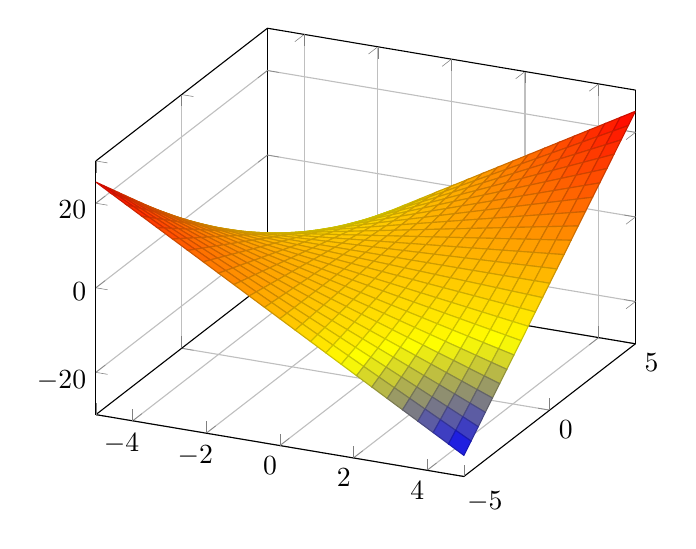
\begin{tikzpicture}
          \begin{axis}[grid=both]
            \addplot3[surf,shader=faceted] {x*y};
          \end{axis}
        \end{tikzpicture}
      }
    \end{center}
  \end{frame}
  
  
  \begin{frame}{Maps}
  
    \begin{alertblock}{Definition of map}
      A map from a set $A$ to a set $B$ is a subset $M$ of $A \times B$ where each element of $A$ appears as the first element of a tuple in $M$ exactly once.
    \end{alertblock}
  
    \redmath{A = \{a,b,c\} \qquad B = \{x,y,z\}}
  
    \begin{minipage}[t]{0.48\linewidth}
    \begin{exampleblock}{Maps}
      \begin{itemize}
        \item $\{(a,x),(b,x),(c,x)\}$
        \item $\{(a,x),(b,y),(c,z)\}$
      \end{itemize}
    \end{exampleblock}
  \end{minipage}
  \begin{minipage}[t]{0.48\linewidth}
    \begin{exampleblock}{Not maps}
      \begin{itemize}
        \item $\{(a,x),(a,y),(b,x),(c,x)\}$
        \item $\{(a,x),(b,y)\}$
      \end{itemize}
    \end{exampleblock}
  \end{minipage}
  \end{frame}
  
  
  
  \begin{frame}{Languages}
    \begin{description}
      \setlength\itemsep{6mm}
      \item[Alphabet:] finite set of symbols, denoted \( \Sigma \).
      \item[String:] tuple \( w \) over \( \Sigma \).
      \item[Star:] all strings over \( \Sigma \), denoted \( \Sigma^* \).
      \item[Language:] subset \( L \) of \( \Sigma^* \).
      \item[Length:] of a string, denoted \( |w| \).
    \end{description}
  \end{frame}
  
  
  \begin{frame}[fragile]{Deciding PRIMES}
    Is there an algorithm that decides if an arbitrary natural number is a prime number?
  
    \red{Yes --- there are many algorithms such as trial division.}
  
    \vspace{8mm}
  
    \hrule
  
    \begin{minted}{python}
  for i in range(2, n):
    if n % i == 0:
      return False
  return True
    \end{minted}
    
    \hrule
  
     \vspace{8mm}
  
    \red{Agrawal, Kayal and Saxena 2002 showed that PRIMES is in P.}
  
  \end{frame}
  
  
  
  \begin{frame}{An undecidable language}
    
    \begin{itemize}
      \setlength\itemsep{6mm}
      \item Encode all Turing machines as strings over $\{0, 1\}$.
      \item Consider the subset of Turing machines that don't ever get stuck in an infinite loop irrespective of the input.
      \item This set is undecidable.
    \end{itemize}
  
  \end{frame}
  
  
  \begin{frame}{SAT}
    
    \red{Example propositional formula: $(A \lor B) \wedge (\neg A \lor \neg C)$.}
  
    \vspace{6mm}
  
    \begin{description}
      \item[Variables:] $A, B, C, \ldots$ -- boolean.
      \item[Operations:] AND ($\wedge$), OR ($\lor$), NOT ($\neg$).
      \item[Brackets:] $()$. 
    \end{description}
  
    \vspace{6mm} 
  
    A formula is satisfiable if there is any values for the variables that makes the formula True.
  
    \vspace{6mm}
  
    \red{Boolean Satisfiability Problem (SAT): $\{ w : w \mathrm{\  is \  satisfiable }\}$.}
  
  \end{frame}
  
  
  \begin{frame}{Turing machines recap}
    For a given input a Turing machine does one of three things:
    \vspace{4mm}
    \begin{description}
      \setlength\itemsep{6mm}
      \item[Accepts] the input string by finishing in the accept state in a finite number of steps.
      \item[Rejects] the input string by finishing in the reject/fail state in a finite number of steps.
      \item[Continues] indefinitely in some sort of infinite loop.
    \end{description}
    \vspace{4mm}
    Remember there are a finite number of states and tape symbols.
  \end{frame}
  
  
  \begin{frame}{Deciders}
    \redmath{f: \Sigma^* \rightarrow \{ q_f, q_a \}}
    \vspace{2mm}
    \begin{description}
      \setlength\itemsep{6mm}
      \item[Decider:] a Turing machine that always finishes in a finite number of steps.
      \item[Decides:] decides the language it accepts.
      \item[Decidable:] a language is called decidable if any Turing machine decides it.
    \end{description}
    \vspace{2mm}
    \red{Important question: are all languages decidable?}
  \end{frame}

  \end{document}